\documentclass{beamer}
\usepackage{movie15}
\usepackage{multirow}
\usepackage{amsmath}
\usepackage{amsthm,amsthm}
\usepackage{amssymb}

\global\long\def\ev{\mathbb{E}}
\usetheme{metropolis}           % Use metropolis theme
\title{ A Kernel Test of Goodness of Fit}
\date{\today}
\author{Kacper Chwialkowski$^*$, Heiko Strathmann$^*$, Arthur Gretton}
\institute{}
\titlegraphic{
    %
\includegraphics[width=2cm]{csml_logo_vector2.pdf}\hspace*{4.75cm}~%
   
\includegraphics[width=2cm]{./img/csml_logo_vector2.pdf}
}

\definecolor{mpigreen}{rgb}{0,0.31,0}


\definecolor{1}{rgb}{ 0.9000,0.4909,0}
\definecolor{2}{rgb}{ 0.8182 ,   0.9000,         0}
\definecolor{3}{rgb}{ 0.3273,    0.9000    ,     0}
\definecolor{4}{rgb}{    0  ,  0.9000 ,   0.1636}
\definecolor{5}{rgb}{   0  ,  0.9000  ,  0.6545}
\definecolor{6}{rgb}{   0  ,  0.6545   , 0.9000}
\definecolor{7}{rgb}{  0  ,  0.1636 ,   0.9000}
\definecolor{8}{rgb}{ 0.3273  ,       0  ,  0.9000}
\definecolor{9}{rgb}{ 0.8182  ,       0  ,  0.9000}
\definecolor{10}{rgb}{  0.9000  ,       0  ,  0.4909}



\newtheorem{thm}{Theorem}



\begin{document}
\frame{\titlepage}
  \setbeamercolor{background canvas}{bg=white}
 \begin{frame}{What is one sample testing?}
 \begin{center}
$\theta_{1}\sim{\cal N}(0,10);\theta_{2}\sim{\cal N}(0,1)$\\
$ X_{i}\sim\frac{1}{2}{\cal N}(\theta_{1},4)+\frac{1}{2}{\cal N}(\theta_{1}+\theta_{2},4) $.
 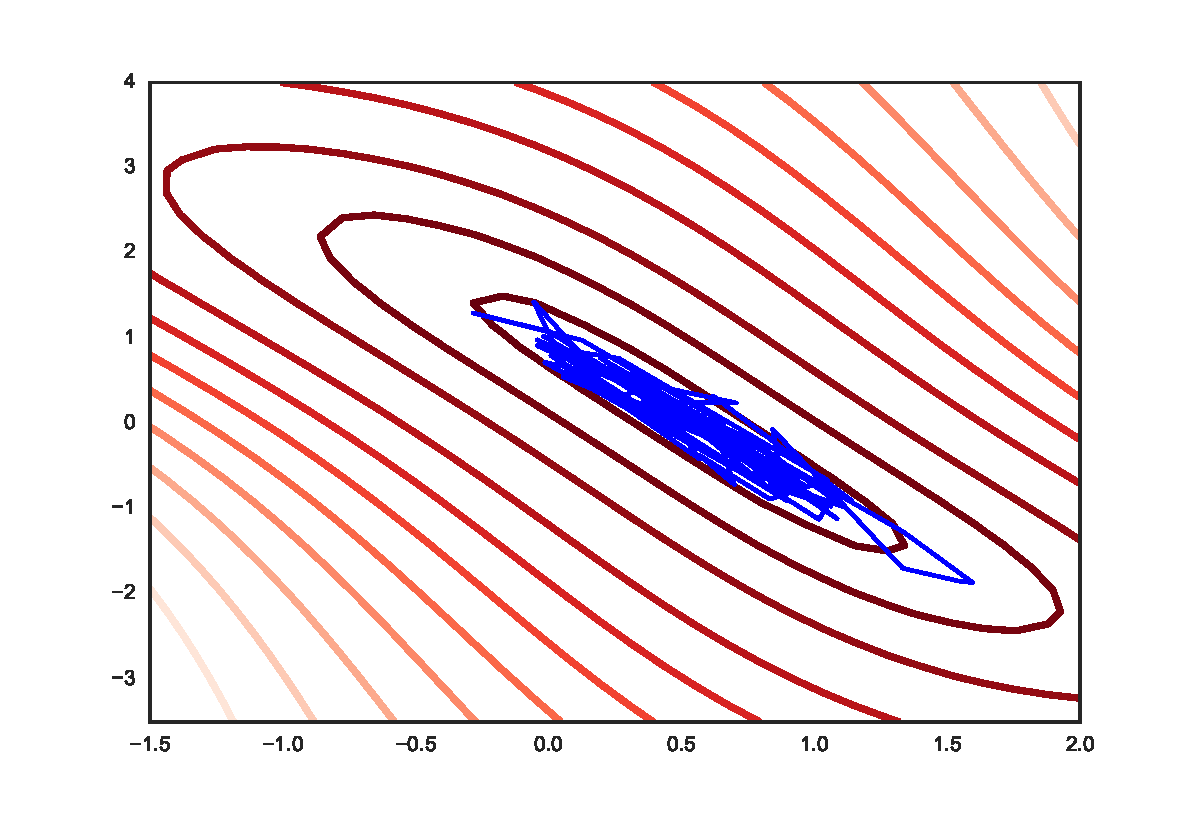
\includegraphics[width=0.6\textwidth]{./img/sgld_trace_and_density.pdf} 
 \end{center}
 \end{frame}
 
 \begin{frame}{Maximum mean discrepancy}
 \begin{center}
$MMD({\color{red} p},{ \color{blue} q},F) = \sup_{ f\in F} [\ev_{{ \color{blue} q}}f - \ev_{{\color{red} p}} f]  $\\
\vspace{0.5cm}
 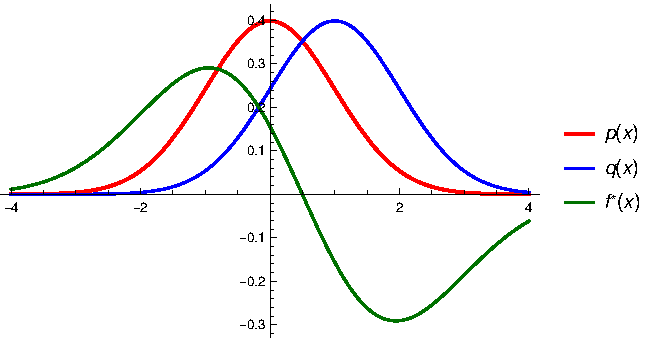
\includegraphics[width=0.6\textwidth]{./img/mmd.pdf} 
 \end{center}
 \end{frame} 
 
 
 
 \begin{frame}{Main idea (by Stein)}
To get rid of $\ev_{{\color{red} p}}f$  in $$ \sup_{f \in F} [\ev_{{ \color{blue} q}}f - \ev_{{\color{red} p}} f ] $$we will use the cornerstone of modern ML

\pause
\textbf{integration by parts}

\pause 
not the chain rule

\pause
I got you

\pause 
\begin{flushright}
\small \textit{Kacper} 
\end{flushright}



\end{frame} 

  \begin{frame}{Cornerstone of modern ML: integration by parts}
  \begin{center}
  Consider the  class  \scalebox{1.3}{ $G = \{ f  +  \log' { \color{blue} q} \cdot  f | f \in F \}$} justified by 
\begin{align*}
 0= &  f(x) {\color{red} p}(x)  \big|_{x=-\infty}^{x=\infty} \\
   = &  \int_{-\infty}^{\infty} (f(x) {\color{red} p}(x) )'  dx \\
   = &  \int   f(x)' { \color{blue} q}(x)   + f(x){\color{red} p}'(x)  \\
   = &  \ev_{\color{red} p} f(X)  +  \log' {\color{red} p}(X) f(X) \\
   = & \ev_{\color{red} p} g(X), \\
    & \quad \quad \quad  \quad  \text{ where } g \in G
\end{align*}
\end{center}

 \end{frame} 
  

 \begin{frame}{Stein discrepancy }
 \begin{center}
 \scalebox{0.8}{ $G = \{ f  +  \log' {\color{red} p} f | f \in F \}$}
 
$MMD({\color{red} p},{ \color{blue} q},G) = \sup_{g\in G} \ev_{{ \color{blue} q}}g - \ev_{{\color{red} p}} g - = \sup_{g \in G} \ev_{{ \color{blue} q}} g $  \\
\vspace{0.5cm}
 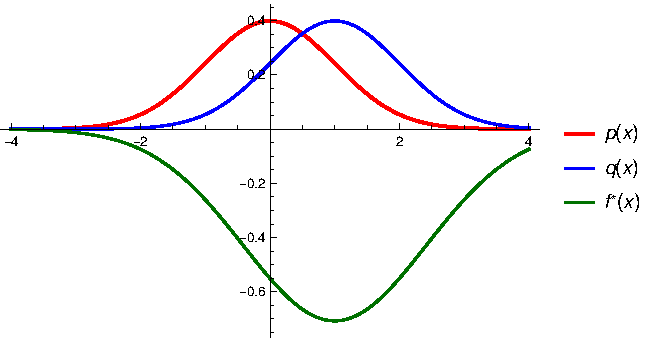
\includegraphics[width=0.6\textwidth]{./img/s1.pdf} 
 \end{center}
 \end{frame} 
  
  
 \begin{frame}{Stein discrepancy}
 \begin{center}
 \scalebox{0.8}{ $G = \{ f  +  \log' {\color{red} p} f | f \in F \}$}
 
$MMD({\color{red} p},{ \color{blue} q},G) = \sup_{g\in G} \ev_{{ \color{blue} q}}g - \ev_{{\color{red} p}} g - = \sup_{g \in G} \ev_{{ \color{blue} q}} g $  \\
\vspace{0.5cm}
 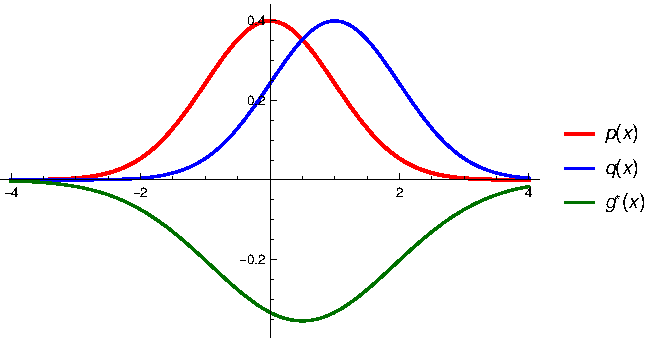
\includegraphics[width=0.6\textwidth]{./img/s05.pdf} 
 \end{center}
 \end{frame} 
 
 
 \begin{frame}{Stein discrepancy}
 \begin{center}
 \scalebox{0.8}{ $G = \{ f  +  \log' {\color{red} p} f | f \in F \}$}
 
$MMD({\color{red} p},{ \color{blue} q},G) = \sup_{g\in G} \ev_{{ \color{blue} q}}g - \ev_{{\color{red} p}} g - = \sup_{g \in G} \ev_{{ \color{blue} q}} g $  \\
\vspace{0.5cm}
 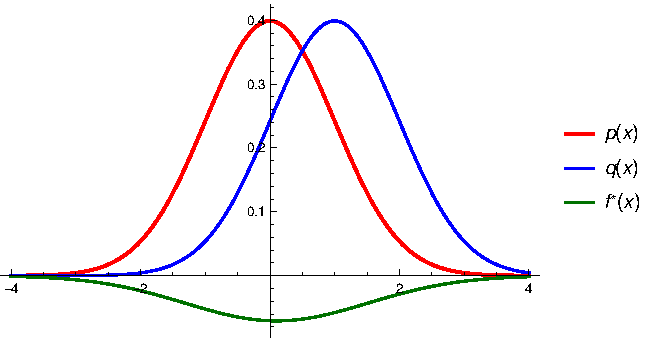
\includegraphics[width=0.6\textwidth]{./img/s01.pdf} 
 \end{center}
 \end{frame} 

 
\begin{frame}{Main results}
\begin{center}
 Let $F$ be the RKHS associated with the kernel $k$. Consider a friendly looking function
\begin{align*}
h_{{\color{red} p}}(x,y) & := \partial_{x} \log {\color{red} p}(x) \partial_{x} \log {\color{red} p}(y) k(x,y)\\
 & \quad+\partial_{y} \log {\color{red} p}(y) \partial_{x}  k(x,y)\\
 & \quad+\partial_{x} \log {\color{red} p}(x) \partial_{y}k(x,y)\\
 & \quad+\partial_{x} \partial_{y} k(x,y).
\end{align*}
\end{center}
\end{frame}
 
\begin{frame}{Main results}

Let ${ \color{blue} q},{\color{red} p}$ be probability measures and $Z\sim { \color{blue} q}$. 
\begin{thm}
If $\ev_{{ \color{blue} q}} h_{{\color{red} p}}(Z,Z)<\infty$, then $MMD({\color{red} p},{ \color{blue} q},G) = \ev_{{ \color{blue} q}} h_{{\color{red} p}}(Z,Z')$.
\end{thm}
\begin{thm}
 If the kernel $k$ is cc-universal, $\ev_{{ \color{blue} q}} h_{{ \color{blue} q}}(Z,Z)<\infty$ and $\ev_{{ \color{blue} q}} (\log' \frac{{\color{red} p}(Z)}{{ \color{blue} q}(Z)})^{2}<\infty$
then $MMD({\color{red} p},{ \color{blue} q},G) =0$ if and only if ${\color{red} p}={ \color{blue} q}$.
\end{thm}

\end{frame} 


 
 \begin{frame}{$V$-statistics}
An estimator of $\ev h_{\color{red} p}(X,X')$ is
\[
 V_n(h_{\color{red} p}) = \frac {1} {n^2} \sum_{i,j=1}^n h_{\color{red} p}(X_i,X_j).
\]
Our test statistic is $ n V_n(h_{\color{red} p})$.

If $X_i \sim {\color{red} p}$ then $ n V_n(h_{\color{red} p})$  converges weakly. 

Otherwise it does not,  it explodes, $P(n V_n(h_{\color{red} p}) <C) \to 0$.
 \end{frame}
 
 
  \begin{frame}{$V$-statistics}
To estimate quantiles of $ V_n(h_{\color{red} p})$  
\[
 V_n(h_{\color{red} p}) = \frac {1} {n^2} \sum_{i,j=1}^n h_{\color{red} p}(X_i,X_j).
\]
under the null, we use wild bootstrap
\[
 B_n(h_{\color{red} p}) = \frac {1} {n^2} \sum_{i,j=1}^n W_i W_j h_{\color{red} p}(X_i,X_j).
\]
  where $W_i$ is a specific series of zero valued random variables.
\end{frame}

 \begin{frame}{Wild bootstrapping}
 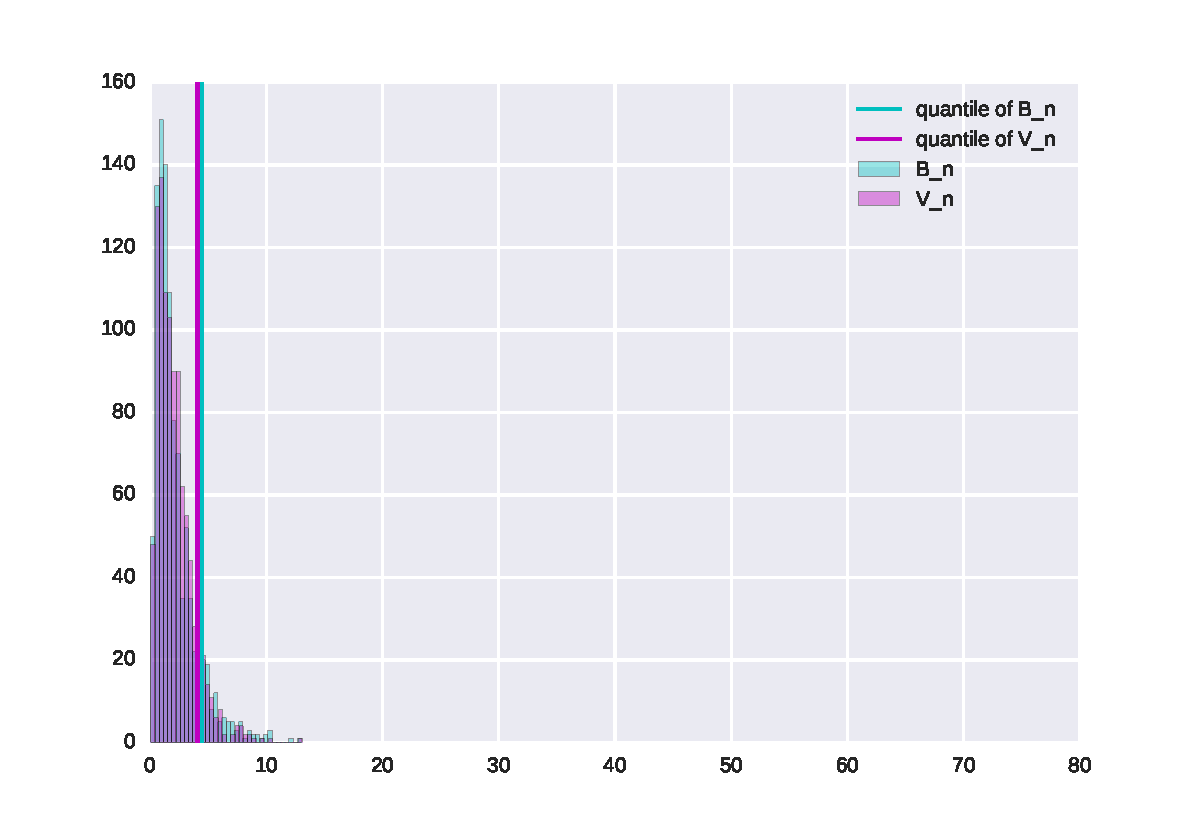
\includegraphics[width=0.9\textwidth]{./img/bootstrapWorks1.pdf}
\end{frame}

 \begin{frame}{Wild bootstrapping}
 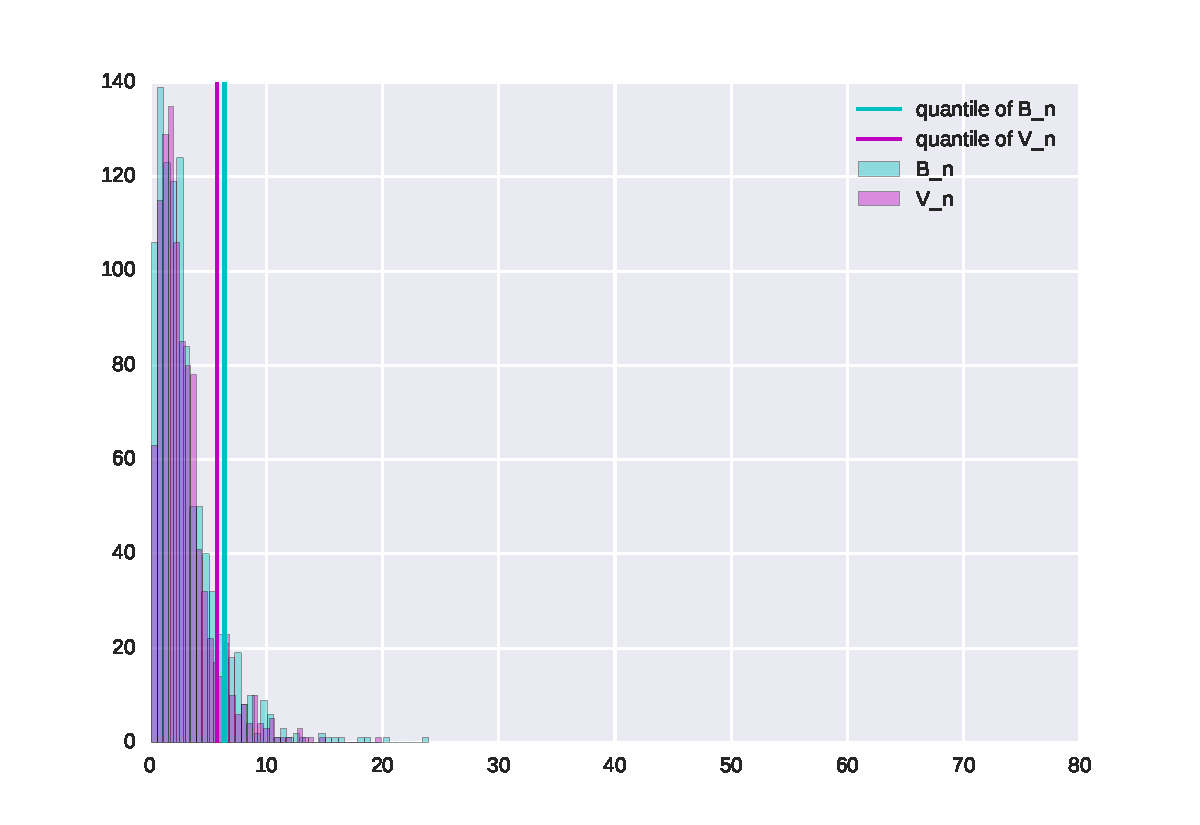
\includegraphics[width=0.9\textwidth]{./img/bootstrapWorks4.pdf}
\end{frame}

 \begin{frame}{Wild bootstrapping}
 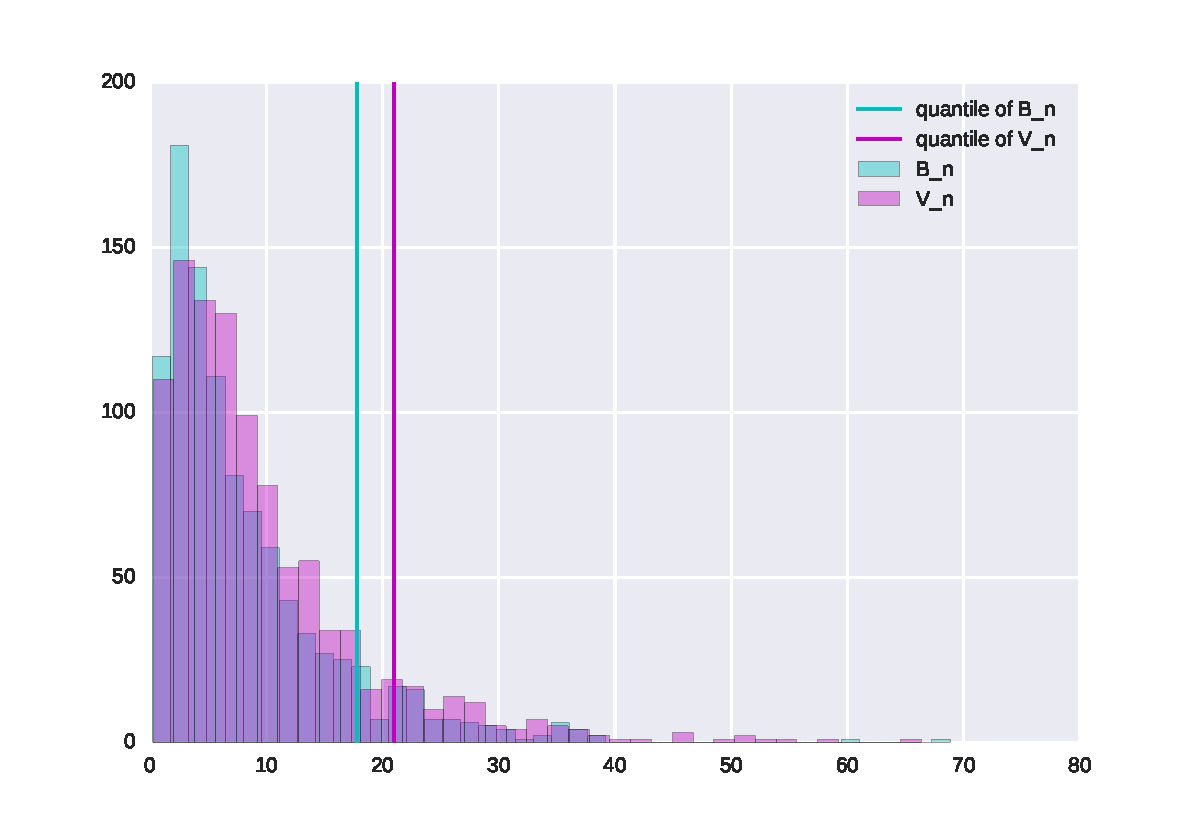
\includegraphics[width=0.9\textwidth]{./img/bootstrapWorks8.pdf}
\end{frame}



  \begin{frame}{Student's t vs.~Normal}
\begin{columns}
        \begin{column}{.5\textwidth}
        \begin{figure}
           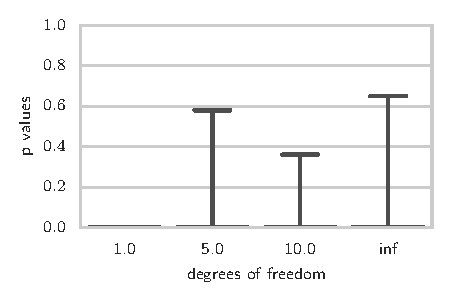
\includegraphics[width=\textwidth]{img/sgld_student_bad} 
           
           
            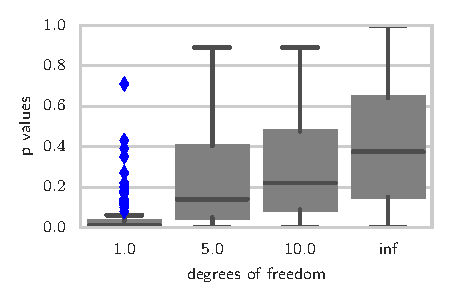
\includegraphics[width=\textwidth]{img/sgld_student} 
        \end{figure}
        \end{column}
        \begin{column}{.5\textwidth}
            \begin{figure}
           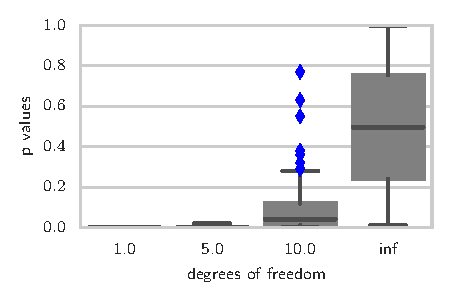
\includegraphics[width=\textwidth]{img/sgld_student_opt} 
        \end{figure}
       Null -- samples are from normal distribution. Draws from the Student's t distribution exhibit temporal correlation.
        \end{column}
    \end{columns}
 

\end{frame}



  \begin{frame}{Bias quantification in Approximate MCMC}
\begin{columns}
        \begin{column}{.55\textwidth}
        \begin{figure}
           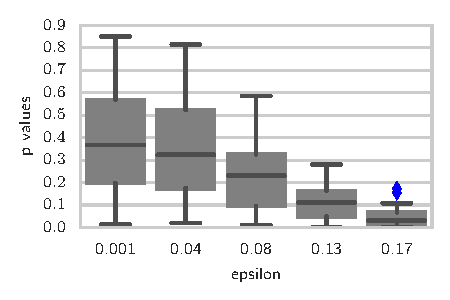
\includegraphics[width=\textwidth]{img/Heiko1} 
           
            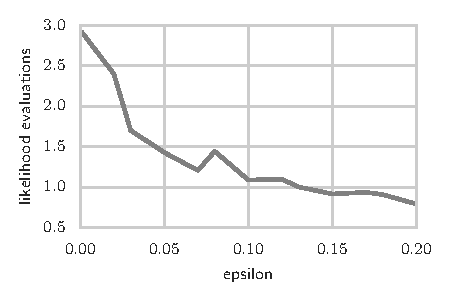
\includegraphics[width=\textwidth]{img/Heiko2}
        \end{figure}
        \end{column}
        \begin{column}{.45\textwidth}
        \begin{align*}
\theta_{1}\sim{\cal N}(0,10);\theta_{2}\sim{\cal N}(0,1)\\
X_{i}\sim\frac{1}{2}{\cal N}(\theta_{1},4)+\frac{1}{2}{\cal N}(\theta_{1}+\theta_{2},4) & .
\end{align*}

            \begin{figure}
           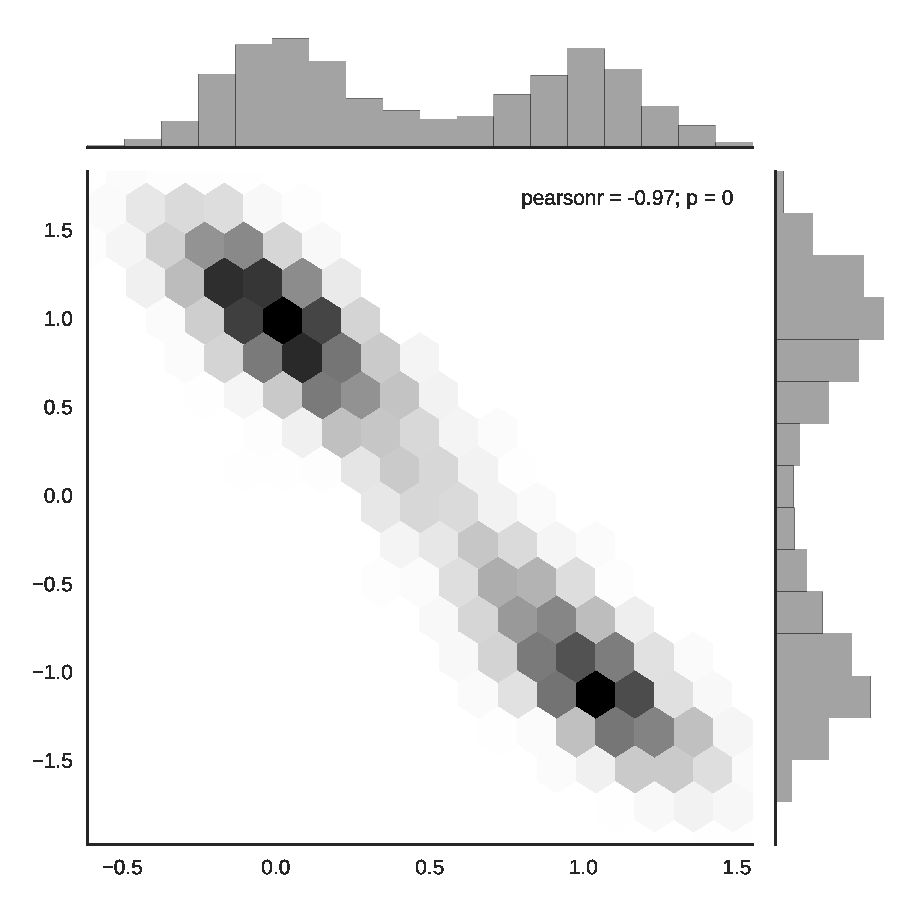
\includegraphics[width=\textwidth]{img/sgld_sample} 
        \end{figure}

        \end{column}
    \end{columns}
 \end{frame}

  \begin{frame}{Experiment 3}
\begin{columns}
        \begin{column}{.5\textwidth}
        \begin{figure}
           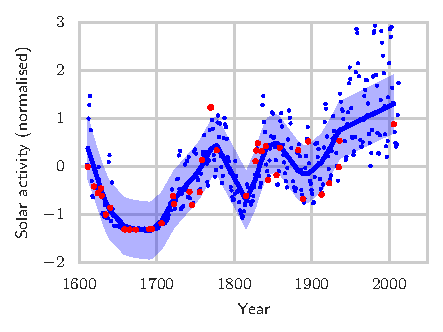
\includegraphics[width=\textwidth]{img/gp_regression_data_fit} 
             
             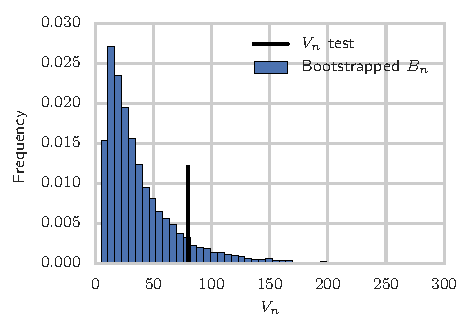
\includegraphics[width=\textwidth]{img/gp_regression_bootstrap_hist} 
        \end{figure}
        \end{column}
        \begin{column}{.5\textwidth}
       We use the \texttt{solar} dataset. We fit $N_{\text{train}}=361$
data using a GP, and perform  maximum likelihood. We then apply our test
to the remaining $N_{\text{test}}=41$ data.
        \end{column}
    \end{columns}
 
 \end{frame}


\end{document}